%% abtex2-modelo-trabalho-academico.tex, v-1.9.6 laurocesar
%% Copyright 2012-2016 by abnTeX2 group at http://www.abntex.net.br/
%%
%% This work may be distributed and/or modified under the
%% conditions of the LaTeX Project Public License, either version 1.3
%% of this license or (at your option) any later version.
%% The latest version of this license is in
%%   http://www.latex-project.org/lppl.txt
%% and version 1.3 or later is part of all distributions of LaTeX
%% version 2005/12/01 or later.
%%
%% This work has the LPPL maintenance status `maintained'.
%%
%% The Current Maintainer of this work is the abnTeX2 team, led
%% by Lauro César Araujo. Further information are available on
%% http://www.abntex.net.br/
%%
%% This work consists of the files abntex2-modelo-trabalho-academico.tex,
%% abntex2-modelo-include-comandos and abntex2-modelo-references.bib
%%

% ------------------------------------------------------------------------
% ------------------------------------------------------------------------
% abnTeX2: Modelo de Trabalho Academico (tese de doutorado, dissertacao de
% mestrado e trabalhos monograficos em geral) em conformidade com
% ABNT NBR 14724:2011: Informacao e documentacao - Trabalhos academicos -
% Apresentacao
% ------------------------------------------------------------------------
% ------------------------------------------------------------------------

\documentclass[
	% -- opções da classe memoir --
	12pt,				% tamanho da fonte
%	openright,			% capítulos começam em pág ímpar (insere página vazia caso preciso)
%	twoside,			% para impressão em recto e verso. Oposto a oneside
    oneside,			% Oposto a twoside
	a4paper,			% tamanho do papel.
	% -- opções da classe abntex2 --
	%chapter=TITLE,		% títulos de capítulos convertidos em letras maiúsculas
	%section=TITLE,		% títulos de seções convertidos em letras maiúsculas
	%subsection=TITLE,	% títulos de subseções convertidos em letras maiúsculas
	%subsubsection=TITLE,% títulos de subsubseções convertidos em letras maiúsculas
	% -- opções do pacote babel --
	english,			% idioma adicional para hifenização
	french,				% idioma adicional para hifenização
	spanish,			% idioma adicional para hifenização
	brazil				% o último idioma é o principal do documento
	]{abntex2}

% ---
% Pacotes 
% ---
\usepackage{lmodern}			% Usa a fonte Latin Modern			
\usepackage[T1]{fontenc}		% Selecao de codigos de fonte.
\usepackage[utf8]{inputenc}		% Codificacao do documento (conversão automática dos acentos)
\usepackage{lastpage}			% Usado pela Ficha catalográfica
\usepackage{indentfirst}		% Indenta o primeiro parágrafo de cada seção.
\usepackage{color}				% Controle das cores
\usepackage{graphicx}			% Inclusão de gráficos
\usepackage{microtype} 			% para melhorias de justificação
\usepackage{filecontents}       % Used so that the external files can be placed in this file

\usepackage[brazilian,hyperpageref]{backref}	 % Paginas com as citações na bibl
\usepackage[alf]{abntex2cite}	% Citações padrão ABNT

% ---
% CONFIGURAÇÕES DE PACOTES
% ---

% ---
% Configurações do pacote backref
% Usado sem a opção hyperpageref de backref
\renewcommand{\backrefpagesname}{Citado na(s) página(s):~}
% Texto padrão antes do número das páginas
\renewcommand{\backref}{}
% Define os textos da citação
\renewcommand*{\backrefalt}[4]{
	\ifcase #1 %
		Nenhuma citação no texto.%
	\or
		Citado na página #2.%
	\else
		Citado #1 vezes nas páginas #2.%
	\fi}%
% ---
\newcommand{\basePath}{/var/www/html/baladecoco/monografia/latex}

% ---
% Informações de dados para CAPA e FOLHA DE ROSTO
% ---
\titulo{Site e-commerce para empresa do ramo alimentício}
\autor{Renan Marcel Ferreira Dias}
\local{Brasil}
\data{Junho de 2017}
\orientador{André Bernardi}
\instituicao{%
  Universidade Federal de Itajubá -- UNIFEI
  \par
  Instituto de Engenharia de Sistemas e Tecnologia da Informação
  \par
  Engenharia da Computação}
\tipotrabalho{Trabalho Final de Graduação}
% O preambulo deve conter o tipo do trabalho, o objetivo,
% o nome da instituição e a área de concentração
\preambulo{Monografia referente ao Trabalho Final de Graduação do curso de Engenharia da Computação da Universidade Federal de Itajubá}
% ---



% ---
% Configurações de aparência do PDF final

% alterando o aspecto da cor azul
\definecolor{blue}{RGB}{41,5,195}

% informações do PDF
\makeatletter
\hypersetup{
     	%pagebackref=true,
		pdftitle={\@title},
		pdfauthor={\@author},
    	pdfsubject={\imprimirpreambulo},
	    pdfcreator={LaTeX with abnTeX2},
		pdfkeywords={abnt}{latex}{abntex}{abntex2}{trabalho acadêmico},
		colorlinks=true,       		% false: boxed links; true: colored links
    	linkcolor=blue,          	% color of internal links
    	citecolor=blue,        		% color of links to bibliography
    	filecolor=magenta,      		% color of file links
		urlcolor=blue,
		bookmarksdepth=4
}
\makeatother
% ---

% ---
% Espaçamentos entre linhas e parágrafos
% ---

% O tamanho do parágrafo é dado por:
\setlength{\parindent}{1.3cm}

% Controle do espaçamento entre um parágrafo e outro:
\setlength{\parskip}{0.2cm}  % tente também \onelineskip

% ---
% compila o indice
% ---
\makeindex
% ---

% ----
% Início do documento
% ----
\begin{document}

% Seleciona o idioma do documento (conforme pacotes do babel)
%\selectlanguage{english}
\selectlanguage{brazil}

% Retira espaço extra obsoleto entre as frases.
\frenchspacing

% ----------------------------------------------------------
% ELEMENTOS PRÉ-TEXTUAIS
% ----------------------------------------------------------
% CAPA ---------------------------------------------------------------------- %
\imprimircapa

% FOLHA DE ROSTO ------------------------------------------------------------ %
\imprimirfolhaderosto*

% DEDICATORIA --------------------------------------------------------------- %
\begin{dedicatoria}
  %% Dedicatória

\vspace*{\fill}
\centering
\noindent
Dedico este tabalho ao meu bebê que está por vir. Sendo Alice ou Samuel, é e será a o bebê, a criança, a pessoa mais amada deste mundo.
\vspace*{\fill}

  % Dedicatória

\vspace*{\fill}
\centering
\noindent
Dedico este tabalho ao meu bebê que está por vir. Sendo Alice ou Samuel, é e será a o bebê, a criança, a pessoa mais amada deste mundo.
\vspace*{\fill}

\end{dedicatoria}

% AGRADECIMENTOS ------------------------------------------------------------ %
\begin{agradecimentos}
  % Agradecimentos

Agradeço a todos os amigos envolvidos em todo o processo deste trabalho e também a todos os desenvolvedores da comunidade Drupal, que trabalham termos um software livre de qualidade. Agradeço também aos meus pais, que sempre me incentivaram a seguir um objetivo com determinação e ajudaram em todas as conquistas. Agradeço especialmente a minha esposa Renata, que me ajudou pacientemente, corrigindo, dando idéias e mantendo meu foco nos objetivos, não só deste projeto, mas de todos os outros, passados, presentes e tenho certeza que nos futuros também.

\end{agradecimentos}

% EPIGAFE ------------------------------------------------------------------- %
\begin{epigrafe}
  % Epigrafe

\vspace*{\fill}
\begin{flushright}
    \textit{``Não vos amoldeis às estruturas deste mundo, \\
    mas transformai-vos pela renovação da mente, \\
    a fim de distinguir qual é a vontade de Deus: \\
    o que é bom, o que Lhe é agradável, o que é perfeito.\\
    (Bíblia Sagrada, Romanos 12, 2)}
\end{flushright}

\end{epigrafe}

% RESUMO -------------------------------------------------------------------- %
\setlength{\absparsep}{18pt} % ajusta o espaçamento dos parágrafos do resumo
\begin{resumo}
  % Resumo

Este é um projeto de um sistema web de e-commerce, construido para uma empresa real do ramo alimentício com base na cidade de Itajubá em Minas Gerais. O objetivo é criar um site rápido e seguro, que entregue ao usuário uma experiência única e apresente de forma clara e informativa o produto da empresa. Alguns conteúdos serão criados para enriquecer o site e chamar a atenção do cliente para o produto.

Utilizaremos o framework e gerenciador de conteúdos Drupal construido na linguagem PHP, escolhido por sua solidez e grande comunidade de desenvolvedores. Sua versão mais recente, o Drupal 8, é uma plataforma flexivel e inovadora, com sistemas de cache bem robustos e várias API's que fornecem métodos seguros de construir um website.

Nossos objetivos poderão ser atingidos com a ajuda de módulos da comunidade Drupal e as mais novas tecnologias e tecnicas de sistemas web que forem cabíveis. O fluxo de desenvolvimento será o mais seguro para a solidez do código, utilizando o software Vagrant para garantir ambiêntes constantes e git para controle de versão. O automatizador de tarefas Gulp e os gerenciadores de pacotes NPM e Composer serão algumas das ferramentas utilizadas para facilitar os processos de instalação e programação.

Esperamos que site tenha um desempenho acima da média e testes são feitos constantemente para garantir este quesito. A mais utilizada será o GTMetrix, ferramenta de teste de performance mais completa atualmente, que ainda dá dicas de pontos para  se melhorar.

\textbf{Palavras-chave}: e-commerce. drupal. web. php. performance. seo. twig. less.

\end{resumo}

% RESUMO EM INGLES ---------------------------------------------------------- %
\begin{resumo}[Abstract]
  % Resumo em ingles

\begin{otherlanguage*}{english}
   This is the english abstract.

   \vspace{\onelineskip}

   \noindent
   \textbf{Keywords}: latex. abntex. text editoration.
\end{otherlanguage*}

\end{resumo}

% ---
% inserir lista de ilustrações
% ---
\pdfbookmark[0]{\listfigurename}{lof}
\listoffigures*
\clearpage
% ---

% ---
% inserir lista de tabelas
% ---
\pdfbookmark[0]{\listtablename}{lot}
\listoftables*
\clearpage
% ---

% ---
% inserir lista de abreviaturas e siglas
% ---
\begin{siglas}
  \item[ABNT] Associação Brasileira de Normas Técnicas
  \item[abnTeX] ABsurdas Normas para TeX
\end{siglas}
% ---

% ---
% inserir o sumario
% ---
\pdfbookmark[0]{\contentsname}{toc}
\tableofcontents*
\clearpage
% ---

% ----------------------------------------------------------
% ELEMENTOS TEXTUAIS
% ----------------------------------------------------------
\textual

\chapter{Introdução}

% =========================================================================== %
\section{O Comércio Convencional}

Quando falava-se em comércio à 20 anos atrás, pensavamos em uma estabelecimento comercial, que podiamos nos deslocar até ele, entrar e sermos atendidos por um vendedor. Um lugar onde podiamos ver o produto que queriamos comprar, tocar, analisar sua cor e sentir seu cheiro. Após escolher, pagariamos com dinheiro ou cheque e levariamos para a casa o produto.


% =========================================================================== %
\section{A Internet}

O comércio muda muito sua cara de tempos em tempos, mas nunca tivemos um salto tão grande na forma de comprar e vender mercadorias como nos últimos 20 anos. Desde 1995 quando a Amazon, gigante americana do comércio eletrônico, fez sua primeira venda online, em uma época que o Brasil ainda estava conhecendo a internet, muita coisa mudou. Novas tecnologias nos permitem comprar e vender sem sair do conforto de nossas casas e também à pagar, receber e movimentar dinheiro por dispositívos móveis que estão conectados a internet 24h por dia, sem ter que ir ao banco e enfrentar filas.

Todas estas mudanças fizeram com que as empresas que quisesem continuar no mercado e ter sucesso nos tempos atuais, mudassem sua maneira de fazer negócio. A importância do comércio físico, apesar de grande, está em decadência, e a presença na web é um requisito fundamental. Empresas que são recordistas em vendas em lojas físicas, como por exemplo a Casa Bahia e o Magazine Luiza, investiram e ainda estão investindo pequenas fortunas na criação e manutenção de seus websites e aplicativos móveis.


% =========================================================================== %
\section{E-commerce}

Comércio eletrônico, e-business ou e-commerce são termos usados para definir qualquer tipo de negociação que envolva trasmissão de dados pela internet\cite{WhatIsEcommerce}. Vários tipos de negócios se encacham nesta definição, de sites de venda de camisetas à sistemas online de bancos onde o cliente pode fazer transações e contratar serviços online.

\subsection{Vantagens}

Uma loja online permite a uma empresa vender produtos com um preço diferenciado, beneficiando os compradores. Isso acontece pois seus gastos são menores, principalmente com vendedores e espaços físicos.

No modo tradicional de comércio, uma empresa que queira ter grande visibilidade, tem que desembolsar grandes quantidades de capital para se intalar em lugares estratégicos, onde o fluxo de compradores é grande. Na internet, um site e-commerce de uma empresa pequena tem tantas chances quanto o de uma empresa com maior capacidade financeira. Tudo depende da qualidade e segurança do site e da força do marketing. Com muito pouco capital, faz-se campanhas de marketing online que atingem muito mais pessoas por dia que uma loja física no melhor ponto de comércio do mundo, seja ele onde for. Isso acontece pois na internet não há barreiras geográficas, pode-se comprar e vender para qualquer lugar do mundo.

\begin{itemize}
  \item Facilidade e conforto de fazer compras sem sair de onde está.
  \item Maior disponibilidade de lojas e produtos.
  \item Melhores condições para pesquisa e comparação de preços.
  \item Sem filas ou espera por vendedores ou atendentes livres.
  \item Acesso a produtos de várias regiões do país e do mundo.
  \item Fácil acesso a promoções e cupons de desconto.
  \item Lojas abertas o tempo todo.
  \item 
\end{itemize}

\subsection{Desvantagens}

Nem tudo é perfeito no mundo do e-commerce. Salvo excessões, estas são algumas desvantagens deste tipo de negócio.

\begin{itemize}
  \item Está sujeito a falhas e pode ser vulnerável a ataques.
  \item Em transações com cartões de crédito, há o risco de roubo ou fraudes.
  \item Impossibilita a inspeção física do bem a ser adquirido.
  \item Preço e tempo de entrega podem inviabilizar o negócio.
  \item Dificuldade e demora no retorno ou troca de mercadorias
  \item Nem tudo pode ser vendido online, como por exemplo comidas perecíveis.
  \item Produtos de alto custo como jóias não tem segurança suficiente para serem despachados como encomenda.
  \item Não há o toque pessoal, interação entre cliente e comprador, que pode fazer diferença na concretização de uma venda.
\end{itemize}


% =========================================================================== %
\section{Ambiente de Desenvolvimento}

Existem várias maneiras de se criar um website, com várias linguagens e frameworks disponíveis. Linguagens como PHP, Ruby, Java e C# estão entre as linguagens mais utilizadas \cite{UsageStatistics}. Fazer um website simples do zero não é tarefa difícil. Porém no caso de um e-commerce, onde segurança e usabilidade são fatores chave para o sucesso do negócio, desenvolver em cima de camadas de software que já te proporciona muitas funcionalidades que serão essenciais, segurança contra ataques e falhas, além de uma comunidade de desenvolvedores que disponibiliza código e ajuda, faz desta a melhor opção. Mais adiante, falaremos da escolha deste framework, quais eram as opções e o critério usado para a seleção.

Outra parte importante do desenvolvimento de um website é a escolha de um serviço de hosting\footnote{Hospedagem de Sites - é um serviço que possibilita a pessoas ou empresas com sistemas online a guardar informações, imagens, vídeo, ou qualquer conteúdo acessível por Web}. Servidores existem em várias partes do mundo e para sites de pequeno tráfego podemos encontrar por preços que vão de 100 reais por ano por um servidor compartilhado a 500 reais por ano uma maquina virtual exclusiva. A qualidade do servidor, sua conexão com a internet e localização física podem fazer muita diferença.

Como mais um fator a se considerar, temos o domínio. Domínio é o endereço que o usuário vai usar no browser para utilizar o website. Alguns domínios podem ser contratados em websites especializados de graça, como por exemplo o domínio `.tk` no `site www.dot.tk`. Estes domínios tem pouca visibilidade nos motores de busca e tem pouca confiança dos usuários por não serem amplamente utilizados. No Brasil, os domínios com melhor visibilidade e confiança são o `.com.br` e o `.com`, que por um custo não muito elevado, por volta de 50 reais, podem ser contratados por um ano.

É muito importante para o desenvolvedor de websites, garantir que o código que foi feito, funcione no servidor da mesma maneira que funcionou no ambiênte de desenvolvimento, computador pessoal ou notebook, de todos que participaram do projeto. Para não termos que instalar o mesmo sistema operacional e softwares em todos os computadores que forem utilizados, o uso de uma maquina virtual é a saida. Em uma maquina virtual, com as mesmas configurações do servidor que será utilizado e de fácil replicação nas máquinas de desenvolvimento, este problema é solucionado.

Outra parte esencial para o desenvolvimento de qualquer tipo software, principamente em web, são os softwares gerenciadores de pacotes e automatizadores de tarefas. Gerenciadores de pacotes ajudam na controle das bibliotecas que serão utilizadas e suas versões. Algumas delas já tomam conta de possíveis dependências que estas podem ter e também facilitam o upgrade ou downgrade quando necessários. Automatizadores de tarefas são úteis principalmente no front-end de uma aplicação web. Muitas tarefas como compilação, minificação e manipulação de arquivos podem ser feitas de forma automática, economizando tempo de desenvolvimento e ajudando o programador a focar no código.

% =========================================================================== %
\section{Tecnologias de Web}

Em aplicações web, temos código que executam tanto no servidor, quanto no cliente. O servidor é onde todas as informações estão guardadas em um banco de dados e o código que é executado nesta fase é chamado de back-end. Já no cliente, normalmente um browser, o código é geralmente para melhorar a experiência do usuário, mostrar as informações de forma mais clara, carregar informações dinamicamente sem mudar de página, fazer interações com o usuário e utilizar efeitos em elementos da página. Esta parte é chamada de front-end.

No próximo capítulo, passaremos por todas as tecnologias utilizadas neste projeto, com uma breve explicação de seu objetivo e aplicação.

% =========================================================================== %
\section{SEO, Performance e Segurança}

\subsection{Search Engine Optimization}

Otimização para motores de busca (do inglês) são um conjunto de técnicas utilizadas em websites para melhorar o seu posicionamento em buscadores como o Google, Bing e Yahoo. Esta é uma parte essencial para a empresa que quer ter visibilidade na internet. Quanto mais próximo do topo em motores de busca, maior a chance de usuários clicarem no seu link e visitarem seu website. Hoje em dia existem empresas e proficionais especializados em SEO\sigla{Search Engine Optimization}, dada a importância do assunto.

\subsection{Performance}

O tempo de carregamento e de renderização de um website impactam muito na quantidade de usuários que ele vai reter. Segundo Shaun Anderson\cite{LoadTime}, SEO da empresa MBSA Marketing LTD, cada segundo a mais que um website demora para carregar, a taxa de abandono aumenta cerca de 6\%, chegando a 25\% após 4 segundos. Além da perda de potenciais clientes, sites com performance probre tem seu rankeamento prejudicado em motores de busca. Existem várias ferramentas e softwares que testam a velocidade e dão dicas para melhora-la, como por exemplo o PageSpeed Insights do Google e o YSlow do Yahoo.

\subsection{Segurança}

Quando trabalhamos com cartões de crédito e informações confidenciais de clientes, temos que preocupar com a segurança destes dados. São quatro os principais fatores a se levar em consideração\cite{SecurityEcommerce}:

\begin{itemize}
  \item Privacidade: Todas as informações sensitivas dos clientes devem ser mantidas em bancos de dados seguros e longe do acesso de pessoas e empresas não autorizadas.
  \item Integridade: As informações dos clientes não devem ser modificadas ou adulteradas.
  \item Autenticação: Tanto o website quanto o cliente devem provar suas identidades um ao outro.
  \item Confirmação: É esperado que as informações trocadas sejam verificadas, para ter certeza que foram transmitidas e de forma correta.
\end{itemize}

% =========================================================================== %
\section{O Cliente}

A empresa Menina das Balas de Coco foi fundada 2010 na cidade de Itajubá, Minas Gerais. Seu único produto é a bala de coco, doce típico brasileiro que costuma ser servido em festas de aniversário. O nome da empresa vem de como era conhecida a fundadora na faculdade, onde cursava Letras e vendia suas primeiras balas. A partir dai, foi-se aperfeiçoando as tecnicas de fabricação e melhorando o produto. Hoje a empresa tem mais de 20 sabores de bala de coco que podem ter recheios diversos sabores, além da bala gelada e a original bala bombom, com cobertura de chocolate. Suas principais formas de vendas são redes sociais, Mercado Livre e no loja física.

\chapter{Objetivo}

% =========================================================================== %
\section{Objetivo Geral}

O objetivo deste trabalho é criar um website e-commerce para a empresa Menina das Balas de Coco. O site terá uma area de publicação de notícias, tipo blog e também cadastro de produtos do tipo bala de coco. Deverá ser possível passar por todo o fluxo de compras no site, sendo aceitável um redirecionamento na hora do pagamento, para plataforma especializada. A performace do website deverá ser medida em softwares adequados e o resultado deve ser acima da média. Os dados dos clientes devem ser captados e mantidos de forma segura. Este website deve servir também como um portal de informações sobre a empresa com boa indexação nos mecanismos de busca, para melhor visibilidade na web.

% =========================================================================== %
\section{Objetivo Específico}

\subsection{E-commerce}

Como todo e-commerce, o site deverá ser capaz de guiar o usuário no processo de compra do produto a ser vendido. A facilidade de uso deste mecanismo é fundamental para o sucesso do negócio. Deverá ser possível para o administrador do site cadastrar o produto e todas as suas variantes de sabor, recheio e cobertura, com o preço em Reais (BRL), um texto de apresentação do produto e imagens. Vitrines destes produtos deverão estar em todas as páginas do site, principalmente na homepage. Por ser a principal razão do site, os produtos deverão ter destaque sempre que mostrados, com uma cor que contraste com o tema do site.

% =========================================================================== %
\subsection{Funcionalidades}

\subsubsection{Notícias}
O site deverá possuir um método de postagem de notícias, informações sobre produtos ou a empresa, como um blog.
Este conteúdo terá um título, uma imagem e um corpo que possa conter texto, imagens e videos. Na pagina de descrição deste post, deverá ser possível compartilha-los em redes sociais, como Facebook e Twitter com simples botão. Na página inicial do site, deverá haver uma breve listagem dos posts mais recentes, somente o título e a imagem com link para uma página com o conteúdo completo.

\subsubsection{Baner}
Teremos também um baner na homepage, utilizado em estrutura carrosel. Este baner será uma imagem da largura da tela, com um título e um texto complementar curto sobrepondo esta imagem. O objetivo deste é dar destaque a qualquer tipo de promoção, postagem ou produto do site.

\subsubsection{Usuários}
A aplicação deverá permitir o cadastro de usuários, tanto para identificação na hora da compra, como para a postagem opiniôes e ingresso em lista de e-mail. Será dado como alternativa ao formulário de cadastro o registro por redes sociais, facilitando o processo. O usuário deverá prover pelo menos nome, email e estado para finalizar o cadastro. Ao iniciar o processo de checkout de uma compra, será requisitado informações adicionais que sejam necessárias, como endereço e documentos.

\subsubsection{Review}
Para dar espaço a opiniões sobre o produto para os clientes, teremos a possibilidade de ter link enviado por e-mail para opiniões sobre os produtos que forem comprados. Este e-mail será enviado pelo site e o conteúdo publicado somente com o aval do administrador. Estes conteúdos terão uma vitrine na homepage e serão mostrados nas páginas dos respectivos produtos.

\subsubsection{Opinião}
Além de opinar sobre o produto, o cliente poderá ser requisitado a dar sua opinião sobre a empresa. Esta informação poderá ser utilizada na homepage, filtrada pelo administrador.

\subsubsection{Páginas de FAQ e Contato}
Para facilitar para os clientes e potencialmente diminuir a necessidade de atendimento direto, o site deverá ter uma página com as perguntas mais frequêntes e suas respostas. Este conteúdo deverá ter fácil sistema de cadastro para o administrador e links em lugares de fácil acesso.

% =========================================================================== %
\subsection{Performance e SEO}

Utilizaremos o máximo possível de técnicas para melhorar a performance do site. Ao final, apresentaremos os testes de performance, comparando-o com os sites mais acessados da internet no momento. É esperado que o tempo de carregamento médio do site fique abaixo dos 3 segundos para proporcionar a melhor experiência para o usuário.

Com uma performance boa, teremos o primeiro passo dado para um boa indexação do site nos mecanismos de busca. Utilizaremos e aprenderamos sobre tecnicas como metatags, microdata, estrutura do HTML e midias sociais.

\subsection{Tecnologias}

Como objetivo final, iremos pesquisar e aprender sobre as tecnologias mais utilizadas para desenvolvimento web, o que nos ajudará a atingir todos os outros objetivos citados acima da melhor maneira possível.

\chapter{Método}

Neste capítulo descreveremos as tecnologias utilizadas para o desenvolvimento do projeto.

% =========================================================================== %
\section{Pré desenvolvimento}

\subsection{Hosting}
Como dito anteriormente, temos muitas opções de servidores para instalarmos este e-commerce. Para a escolha, foi levada em consideração a recomendação dos usuários do framework que será utilizado (será explanado na próxima seção) postado em \url{www.drupal.org/hosting}, o preço oferecido, a quantidade de domínios possíveis e o espaço em disco disponibilizado. As melhores opções na época de contatação do serviço eram:

\begin{table}
  \centering
  \begin{tabular}{llll}[Hosting]
    \hline
    Nome      & Espaço    & Domínios  & Valor         \hline
    Bluehost  & Ilimitado & 3         & R\$ 15,90/mês \hline
    Hostgator & Ilimitado & Ilimitado & R\$ 9,99/mês  \hline
    GoDaddy   & Ilimidado & Ilimitado & R\$ 10,99/mês \hline
    SiteGroud & 20 GB     & Ilimitado & R\$ 14,99/mês \hline
  \end{tabular}
  \caption{Opções de hosting para o e-commerce.}
  \label{Hosting}
\end{table}

Deste, foi escolhido o serviço da empresa Hostgator, por oferecer espaço e domínios ilimitados e o menor preço.

\subsection{Domínio}
Como também é um fator importante para SEO, foi sugerido ao cliente escolher um nome de domínio simples, facil de ser associado com a marca e com um top level domain (TLD ou domínio de nível superior) que dê credibilidade ao site como por exemplo o `.com` ou `.com.br`. No caso deste último, a indexação será melhor em uma busca nacional \cite{TLD}. Foi então combinado de usar o nome da empresa com o TLD mais utilizado, com mais de 90\% dos sites brasileiros \cite{RegistroBr}, ficando como a seguir:

\begin{figure}
  \centering
    \large
    meninadasbalas.com.br
\end{figure}

Comprado online na empresa GoDaddy \url{br.godaddy.com}, foi pago R\$ 44,99 por 1 ano de direito de uso deste domínio.

% =========================================================================== %
\section{Drupal}

Como base para o o e-commerce utilizaremos o framework e gerenciador de conteúdo Drupal.  Este software foi criado em 2000 pelo estudante universitário belga Dries Buytaert para ser um pequeno gerenciador de postagem um blog. Mais tarde em 2001, o código deste sistema foi aberto ao público, com o intuito de permitir as pessoas pudessem realizar experimentos e construir extenções. Desde então, o número de usuários vem crescendo a cada ano e sua comunidade de desenvolvedores melhorando o código diarimente. Hoje o Drupal conta com mais de 37 mil extenções \cite{DrupalModules}, chamadas de módulos, com diversas funcionalidades e utilizando as mais novas tecnologias, além de mais de 2 mil temas \cite{DrupalTheme}.

Os motivos desta escolha são:

\begin{itemize}
  \item Segurança: Muitas camadas de proteção são oferecidas pelo Drupal, desde controle de acesso de usuários à API's que protegem o sistema de ataques.
  \item Flexibilidade: Podemos usa-lo para todo e qualquer tipo de site ou serviço online e seu sistema pode ser adaptado para qualquer projeto.
  \item Comunidade: A quantidade e qualidade das extenções providas pela comunidade para adicionar as mais diversas funcionalidades.
  \item Experiencia: Prévia experiência com o framework, o que facilita o design e desenvolvimento do sistema e-commerce.
\end{itemize}

\subsection{Drupal 8}

A versão estável mais recente do Drupal é a número 8 e será a utilizada no projeto. Comparada com a versão anterior, temos um sistema de cache muito mais potênte, módulos importantes adicionados ao núcleo, a mudança do sistema de templates de PHP para Twig, segurança reforçada e novas tecnologias e padrões sendo absorvidos. 

\subsection{Núcleo}

Ao instalar o Drupal nos deparamos com um site cru, mas com várias funciolidades já prontas para serem utilizadas. Algumas delas serão de suma importância para atingirmos nossos objetivos e serão listadas abaixo, pelo nome do módulo no núcleo.

\subsubsection{Node}
O gerênciamento de conteúdo é algo nativo do Drupal, então planejaremos quais os tipos que teremos no site. Cada conteúdo, conhecido como node, pode ter campos configuráveis, que podem representar propriedades do mesmo como por exemplo título, descrição, imagem, relação com outro conteúdo, autor, entre outros. Alguns deles como titulo, autor e status de publicação são padrões para todos.

Planejamos quatro tipos de conteúdo:
\begin{itemize}
  \item Banner - Representando o baner da página inicial, tendo campos para título, um subtítulo e uma imagem.
  \item Review - Representando as opiniôes dos usuários sobre os produtos com um campo de texto e o título automático, para facilitar a criação deste conteúdo.
  \item Article - Postagens gerais de conteúdo aberto, com título, imagens e textos.
  \item Opinion - Representando os opiniôes dos usuários sobre a empresa.
\end{itemize}

Poderiamos considerar o produto também um conteúdo, mas como veremos adiante, este é uma entidade a parte, criada por um módulo da comunidade.

\subsubsection{Taxonomy}
Já pensando nos produtos, criaremos um vocabulário de taxonomia, que é uma lista de keywords utilizadas para organizar o conteúdo do site. Estas keywords serão os sabores de balas que a empresa fabrica e serão atrelados a cada produto, para facilitar a posterior filtragem e exibição destes.

\subsubsection{Views}
Modo mais comum de exibir grupos de conteúdo no Drupal, o módulo Views é um dos que na versão anterior não eram parte core e por sua importancia foi incorporado. Ele permite filtragem e ordenação por valores de propriedades e a exibição de um número específico de conteúdos. 

Com ele, faremos os blocos de baners, reviews, notícias, produtos e opiniões da homepage.
\begin{itemize}
  \item Baner: Os 3 conteúdos do tipo baner em formato de carrosel automático.
  \item Notícias: As 3 notícias mais recentes postadas.
  \item Reviews: Os 4 reviews mais visualizados.
  \item Opiniões: 3 opiniões escolhidas pelo administrador.
\end{itemize}

Além dos blocos, faremos também as páginas de listagem de produtos, reviews, opiniões e notícias.

\subsubsection{User}
Responsável pelo gerenciamento dos usuários do site e suas permissões, este módulo nos permitirá ter usuários logados com todas as informações necessárioas para o fluxo de compras e criação de conteúdo.

\subsubsection{Menu}
Este módulo, como o nome já diz, cria menus com ancoras para outros lugares do site ou sites externos. Segue a listagem dos menus do site, com nome, localização e função:

\begin{itemize}
  \item Topbar Contact Menu: Localizado no topo da página, terá apenas dois links para a página de contato.
  \item Topbar User Menu: Também no top da página, terá links de login e registro para usuários anônimos e links para detalhes da conta e sair para usuários logados.
  \item Main Menu: Menu principal, na parte superior do site com links para as páginas mais importantes.
  \item Footer Menu: No rodapé do site, menu com links para loja, página de contato e informações em geral.
\end{itemize}


% =========================================================================== %
\section{Ambiente de Desenvolvimento}

Com o framework escolhido, vamos construir o ambiênte de desenvolvimento. 

\subsection{Sistemas Operacinais e Maquina Virtual} 
Utilizarei o sistema operacional Ubuntu 16.04 e esporadicamente OSX El Capitan para desenvolvimento local e no servidor temos um CentOS 6. Para evitar problemas de compatibilidade como dito no capítulo de introdução, utilisaremos para desenvolvimento local uma maquina virtual (VM) com as mesmas configurações do servidor. O gerenciamento e configuração desta será feita por um software especializado chamado Vagrant.

Será usada uma configuração pré-definida criada por Jeff Geerling \url{www.drupalvm.com/}, Arquiteto Drupal, especificamente para o Drupal, onde o Vagrant cria uma maquina virtual e a configura especificamente para Drupal, com todos os programas e ferramentas que serão necessárias para o desenvolvimento. Alteramos somentes os pontos onde temos que imitar o servidor Hostgator, que é a versão dos softwares Apache2 e MySQL e a versão da linguagem PHP. Isso já nos garante o funcionamento estável e previsivel do nosso site em todos os ambiêntes que ele estiver instalado.

\subsection{Apache, PHP e MySQL}
Apesar do Drupal funcionar com vários softwares de servidores web, como Nginx e Hiawatha, o mais utilizado é o Apache2. Além disso, nosso servidor também roda Apache2 2.2.25, então este é a escolha inevitável. 

Para a linguagem de servidor, o Drupal 8 requer PHP na versão mínima 5.5.9 e no servidor podemos escolher entre 5.5, 5.6 e 7.0. Foi escolhido a versão 7.0 por ser mais rápida \cite{PHP7Velocidade} e possuir funcionalidades mais avançadas e seguras que a versão 5.6 \cite{PHP7}.

O software de banco de dados será o MySQL versão 5.6.32, que é a única opção no servidor e foi verificada a versão utilizada.

\subsection{Fluxo}
O código será versionado pelo software Git e salvo em repositório publico remoto mantido pela empresa Github \url{www.github.com}. Quando cada pequena tarefa for terminada, um commit é feito com uma breve descrição do que foi feito. Versões de teste serão carregadas para o servidor via SSH (\TODO), também utilizando o Git. Um subdomínio será criado para esta versão de teste, adicionando `dev.` no endereço do site. Esta versão será exclusivamente para testes e deverá ter acesso restrito ao publico em geral. Assim que uma versão estável for atingida, mesmo que sem todos os requisitos do site alcançados, esta será carregada para o ambiente de produção, no domínio principal. O objetivo deste fluxo é ter o máximo de funcionalidades possíves antes de inaugurar o site.

\subsection{Composer}
Iremos utilizar o software gerenciador de pacotes Composer para instalar o Drupal e suas dependências e posteriormente os módulos da comunidade que serão necessários. Uma boa base para o projeto pode ser o Drupal-Composer Project \url{www.github.com/drupal-composer/drupal-project}, código de configuração e scripts do Composer que montam o Drupal com a estrutura de arquivos requirida por ele.

Porém, um problema foi detectado no uso deste pacote. O Drupal é instalado em um sub-diretório do projeto e não na raiz. Isso nos impede de utilizar o domínio principal quando o site for instalado no servidor, pois os arquivos tem que estar na raiz do diretório. Para resolver isto, criei uma fork \TODO \url{https://github.com/renanmfd/drupal-project} deste projeto no Github e modifiquei todos os códigos e configurações para instalar o Drupal no diretório raíz. Esta \TODO fork foi carregada no site Packagist \url{https://packagist.org} para ficar disponível para download via Composer \url{https://packagist.org/packages/renanmfd/drupal-project}.

\TODO comando \$ composer create-project drupal-composer/drupal-project:8.x-dev meninadasbalas --stability dev --no-interaction

Com o problema sanado, podemos dar inicio ao processo de instalação do Drupal e logo após a fase de codificação do projeto.

% =========================================================================== %
\section{Front-end}

\subsection{Bootstrap}
Para o estilo ou tema do site, utilizaremos um dos melhores e mais utilizados frameworks de CSS e Javascript \cite{Bootstrap} que existe atualmente, o Boostrap. A escolha deste se deu simplesmente pelo conhecimento prévio e facilidade de uso. Com ferramentas para design responsivo e bibliotecas Javascript para funcionalidades que serão necessárias como por exemplo o carrosel de baners, este framework é a melhor opção para este projeto. No momento do desenvolvimento deste projeto a versão mais estável é a 3.

\subsection{Temas Drupal}
Na comunidade de Drupal, temos um tema Boostrap, que é uma base para sites que pretendem utilizar esta ferramenta para constriur seus layouts. Este é nosso primeiro requerimento do projeto, instalado via Composer.

\TODO comando \$ composer require drupal/bootstrap

Criaremos um sub-tema, com base no Bootstrap para Drupal que será chamado `MBC Theme`. Neste tema teremos os arquivos de CSS, imagens utilizadas pelo CSS, Javascript, templates Twig e um arquivo de PHP onde podemos modificar e adicionar as variáveis que são passadas os templates. 

Em seguida, para facilitar o desenvolvimento, vamos instalar também um tema administrativo, que como o adjetivo já diz, só é utilizado nas páginas administrativas do site. Foi escolhido o tema Adminimal Theme, por ser um dos temas desta categoria mais utilizados e proporcionar uma interface responsiva e limpa.

\TODO comando \$ composer require drupal/adminimal_theme

\subsection{LESS}
Less é um pré-processador de CSS que extende a linguagem, adicionando melhorias como variáveis, funções e várias outras tecnicas que deixam a manutenção do CSS mais fácil \cite{Less}. Ela foi escolhida por ser utilizada nativamente no framework Bootstrap versão 3.

\TODO Exemplo de LESS -> CSS

O tema do site derá desenvolvido da forma mais modular possível, cada bloco minimo do site tendo seu próprio arquivo, que serão unificados e processados pelo compilador do LESS. A intenção é facilitar a futura melhoria de performance, carregando na página apenas o estilo dos blocos que estão nela. Inicialmente, todos serão incluídos e transformados em um único arquivo de CSS que carregara em todas as páginas.

\subsection{Javascript}
Interações e efeitos mais avançados em páginas web são feitos pelo Javascript (JS), linguagem de script interpretada pelo browser, que tem acesso a toda a estrutura do site. O carrosel de baners na homepage irá utilizar uma das funcionalidades que o JS do framework Bootstrap disponibiliza.

Para garantir qualidade do código JS, utilizaremos a ferramenta ESLint criada por Nicholas C. Zakas em 2013. Esta analiza o código e avisa sobre estruturas que não seguem  padrões de código ou são consideradas inseguras.

\TODO Onde mais tem JS.
\subsection{jQuery}
Para facilitar o desenvolvimento com Javascript e por ser um requerimento do Boostrap, utilizaremos a biblioteca jQuery. Esta possui várias funções que são muito utilizadas no desenvolvimento o que facilita algumas tarefas.

\TODO Exemplo facilidade JS -> jQuery

\subsection{NPM & Gulp}
Para fechar o ambiente de front-end, utilizaremos o automatizador de tarefas Gulp e alguns pacotes de extenção que ele possúi. O Gulp e suas extenções são escritas em Javascript e executam em ambiente do NodeJS. Para instala-los, utilizamos o gerenciador de pacotes do NodeJS chamado Node Package Manager (NPM). Após instalar o NodeJS e o NPM, utilizamos os seguintes comandos para instalar o Gulp e seus pacotes.

\TODO 
# Em qualquer pasta, para instalar o Gulp no sistema e poder utiliza-lo por linha de comando.
$ npm install --global gulp
# Na pasta raiz do tema, inicializamos o projeto npm, que cria um arquivo `package.json` com os dados do projeto.
$ npm init
# Agora instalamos alguns dos pacotes necessários.
$ npm install --save-dev gulp gulp-less gulp-utils gulp-eslint
\TODO comando \$

O Gulp é utilizado via código Javascript, onde utilizamos seus plugins para automatizar tarefas de front-end. As seguintes tarefas serão implementadas:

\begin{itemize}
  \item Less Hint - Ferramenta de análise de código LESS que ajuda na escrita limpa e consistente.
  \item Less Compile - Compila o arquivo principal do LESS, o qual importa todos os outros e gera um CSS minificado e com sourcemap\TODO.
  \item JS Lint - Análise de código JS para evitar estruturas inseguras e garantir que os padrões de código sejam seguidos.
  \item JS Minification - Minificação dos arquivos de de Javascript para melhorar performance.
  \item Image Minification - Minificação do arquivos de imagens do tema também para performance.
  \item Favicon Creation - Criação de uma gama de arquivos de favicon, para que vários tipos de aplicativos, sistemas operacionais e programas tenham o favicon do tamanho correto, a partir de uma  única imagem.
  \item Watch - Escaneia todos os arquivos do tema para mudanças e executa as tarefas especificas ao arquivo que mudou. Por exemplo, a cada vez que um arquivo de LESS for salvo, o arquivo principal é compilado e um novo CSS estará disponível, já com as mudanças salvas.
\end{itemize}

No anéxo 1, temos a lista dos pacotes do NodeJS utlizados e o arquivo de configuração do Gulp.

% =========================================================================== %
\section{Commerce}
O Commerce é um modulo do Drupal para construção de lojas online que pode ser considerado como sendo um framework pelo tamanho e extensividade. Existem vários módulos que extendem o Commerce, adicionando funcionalidades, como por exemplo, diversos metodos de pagamento e serviços de entrega de produtos. Este módulo nos permite criar várias lojas, produtos, tipos de produtos e tipos de variantes de produtos.

\subsection{Produto}
Nosso site terá apenas uma loja. Uma loja extra é necessária quando por exemplo os produtos são enviados de lugares diferentes e produtos deste lugares não podem estar juntos em um pedido, o que não é o nosso caso.

Nosso único tipo de variante de produto será a bala de coco. Variantes são pequenas variações nas propriedade dos produtos podem ser representadas por campos. No caso deste trabalho, a utilização de variantes implicaria em termos somente duas páginas de produtos, a da bala tradicional e da bala recheada, com um formulário para a escolha das características, como se fosse por exemplo uma página de um computador na Amazon, com opções de tamanho de memória RAM. Neste conteúdo teremos campos gerais para as balas, como imagem, preço, descrição e sabor.

Para os tipos de produtos, teremos dois. Um representará a bala tradicional sem campos adicionais e outro a bala recheada com um campo de sabor de recheio. Esta propriedade esta relacionada as diferentes características que um produto pode ter e tem que estar relacionada com um tipo de variante, no nosso caso, a bala de coco.

O produto em si, será o conteúdo final a ser mostrado pela loja, deverá ser de um dos tipos de produto criados e pertencentes a uma ou mais lojas.

Todo este fluxo ajuda o módulo a organizar o e-commerce de modo que a loja seja flexível em relação aos produtos que serão vendidos. No caso deste e-commerce, utilizamos pouco desta flexibilidade por ter apenas dois tipos de produto.

\subsection{Cart}
O Commerce nos proporciona um carrinho de compras atrelado a conta do usuário. Todo produto pode ter um botão para adiciona-lo ao carrinho do usuário ativo. Se for um visitante, o carrinho é guardado do mesmo jeito, porém pelo id da sessão, fazendo deste um carrinho temporário. Tembém temos um bloco para a página inicial com um botão que abre um resumo dos itens selectionado pelo usuário e um link para a página de detalhes do carrinho.

\subsection{Shipping}
Para o sitema de serviço e pagamento da entregas, temos que utilizar uma integração com os correios. Esta integração não existe no Drupal 8, então será algo que iremos criar. Como este é uma parte complicada e deverá tomar um tempo, será utilizado um sitema de pagamento fixo por produto para a entrega, que é nativo do módulo Commerce Shipping e mais adinte, dedicaremos uma seção ao módulo de integração do Commerce, Drupal 8 e a API dos Correios do Brasil.

\subsection{Checkout}
O processo de compra também é gerenciado pelo Commerce. O carrinho, quando o usuário começa o fluxo de compra, é transformado em uma order. O fluxo acontece em 5 etapas:

\begin{itemize}
  \item Identificação: O usuário que não estiver logado, será pedido que entre com seu e-mail e senha ou que registre para uma nova conta no site.
  \item Informações: Nesta etapa será pedido ao usuário informações de contato, dados para envio, tipos e valores de envios e tipo de pagamento a ser utilizado.
  \item Revisão: Todos os dados da compra são exibidos para o usuário conferir os dados.
  \item Pagamento: Será requisitado os dados de pagamento ou haverá um redirecionamento para serviço de pagamento externo.
  \item Completo: Uma mensagem será exibida com o status do pedido e outras informações pertinentes.
\end{itemize}

\subsection{Paypal}
Por ser o método de pagamento mais utilizado mundialmente, o Paypal tem uma integração bem consolidada no Drupal 8 e o módulo Commerce. Por estas razões, ele será a única forma de pagamento para o site inicialmente. Idealmente, gostariamos que o pagamento pudesser ser feito por serviços brasileiros como PagSeguro e MercadoPago, mas a integração destes com o Commerce ainda não existe ou está em desenvolvimento para o Drupal 8.

Para utilizar os serviços do Paypal, instalamos o módulo Commerce Paypal no nosso site, criamos uma conta no site do serviço e requerimos uma chave para sua API. Esta chave é utilizada pelo módulo Commerce para realizar o pagamento dos produtos sem sair do nosso sistema.

% =========================================================================== %
\section{Extendendo o Drupal}

Para continuar a construção das funcionalidades de back-end do site, temos que adicionar módulos da comunidade Drupal. Falaremos agora dos mais importantes e o em qual tarefa eles irão nos auxiliar.

\subsection{Paragraphs}
\subsection{Shield}
\subsection{Social Login}
\subsection{Display Suite}
\subsection{Pathauto}
\subsection{Menu Block}

No anexo \ref{app:modules} temos uma lista de todos os módulos Drupal instalados com uma descrição das suas funcionalidades.

% =========================================================================== %
\section{Performance}

Para termos um site rápido, que retem os clientes do negócio, utilizaremos algumas técnicas e descreveremos algumas que o Drupal 8 já utiliza como padrão.

\subsection{Minificação, Agregação e Compactação}
As mais simples das melhorias que afetam positivamente a performance de um website são a minificação, agregação e a compactação dos recursos que o browser tem que baixar para montar a página. 

A minificação é o processo de remover caractéres desnecessários dos arquivos, normalmente espaços e quebras de linhas e no caso do Javascript, renomeando funções e variáveis com nomes de um só caractere, sem mudar a lógica do script. Após a minificação, os arquivos minificados ainda podem ser utilizados pelo browser normalmente. O benefício é a diminuição do tamanho dos recursos do website.

A agregação é o processo de juntar todos os arquivos com mesma extenção no menor número possivel de arquivos. Por exemplo, todos os recursos de CSS de um site, que no caso do Drupal 8 pode chegar a ser entre 30 e 50, são agregados e transformados em 3 arquivos maiores. Isso melhora a performance por que diminui o numero de requisições o browser tem que fazer para montar a página.

A compactação é um processo que diminui o tamanho do arquivo com tecnicas mais avançadas e requerindo que o browser faça a descompactação antes de utilizar os recursos. É a mesma situação de compactar um arquivo PDF na extenção ZIP, ele diminui o tamanho do arquivo, porém para utiliza-lo novamente temos que descompactar. Esta compactação é feita pelo servidor somente quando ele está habilitado a faze-lo e a requisição possui  um header específico, que avisa a ele que o cliente está apto a receber recursos compactados.

O Drupal 8, em suas configurações, já habilita a compactação dos arquivos pelo servidor. Estas estão no arquivo .htaccess na raíz do projeto.

Apesar do Drupal ter uma funcionalidade de compactação de CSS e JS, vamos instalar um módulo da comunidade que o faz com ferramentas melhores e possúi mais opções, entre elas a agregação de arquivos. Este módulo se chama Advanced Aggregation.

Outro recurso que precisa ser minificado são as imagens do site e para isto utilizaremos o módulo TinyPNG.

\subsubsection{TinyPng}
Este módulo foi desenvolvido originalmente para o Drupal 7, sem versões para o Drupal 8. Por ser um módulo relativamente simples, fizemos a migração e adaptação deste módulo para o Drupal 8. Algumas características não foram implementadas por uma questão de tempo e simplicidade. Este módulo utiliza o serviço do site TinyPNG \url(www.tinypng.com) e sua API para minificar todas as imagens que são carregas no site. O código é bem breve, sendo somente uma função.

\lstset{language=PHP}
\begin{lstlisting}[frame=single]
  <?php

  use Drupal\Core\Entity\EntityInterface;

  /**
   * Implements hook_entity_presave().
   *
   * Process the image with TinyPNG service.
   */
  function tinypng_entity_presave(EntityInterface $entity) {
    $config = \Drupal::config('tinypng.settings');
    if ($entity->isNew() && $entity->getEntityTypeId() == 'file' && empty(file_validate_is_image($entity)) ) {
      $config = \Drupal::config('tinypng.settings');
      $api_key = $config->get('api_key');
      // Skip if no api key is set.
      if (empty($api_key)) {
        drupal_set_message(t('The API key for tinyPNG is not set.'), 'error');
        return;
      }
      // Compress image.
      $image_path = $entity->getFileUri();
      \Tinify\setKey($api_key);
      $dest = drupal_realpath($image_path);

      try {
        if ($config->get('integration_method') == 'download') {
          $origin = file_create_url($image_path);
          $res = \Tinify\fromUrl($origin, $dest);
          $res->toFile($dest);
        }
        else {
          $res = Tinify\fromFile($dest)->toFile($dest);
        }
      }
      catch (Exception $ex) {
        \Drupal::logger('tinypng')->error($ex->getMessage());
      }
    }
  }
\end{lstlisting}

\subsubsection{Blazy}
Mais uma técnica utilizada é o Lazy Load. Esta consiste em adiar o carregamento das imagens de uma página até que ela seja necessária. Se a imagem esta em uma parte visível da página, ela é carregada logo após a renderização do site e não durante. Isso reduz o tempo de carregamento de uma página por que diminui os recursos a serem baixados durante a renderização da página.

Para implementar esta funcionalidade utilizaremos o módulo Blazy do Drupal. Este adiciona formatadores de imagem que trocam o nome do atributo src para data-src da tag HTML img. Isso faz com que o browser não baixe a imagem durante a renderização, por não ter uma atributo src. Após a renderização da página, um código Javascript troca o nome de volta para src, fazendo com que o browser identifique e baixe as imagens necessárias. As que estão em porções não visíveis da tela, este atributo será mudado de nome somente quando esta porção estiver visível.

\subsection{Técnicas}
Uma técnica imprecindível para melhorar a velociadade de um site é fazer com que partes dele que sejam estáticas sejam processadas pelo servidor somente uma vez e seu resultado salvo para ser utilizado em outras requisições. Isso se chama cache. O Drupal 8 possúi um sistema bastante robusto de cache, que pode ser configurado para qualquer site. No nosso caso, utilizaremos as configurações que já vem padrão, somente desabilitando este cache nos ambientes de desenvolvimento.

\subsection{Medição}
A principal ferramenta que iremos utilizar para medir a performance do site é o serviço de análise GTMetrix do site \url{www.gtmetrix.com}. Esta ferramenta da notas a performance do site, baseadas em velocidade, boas práticas, quantidade de requests e tamanho total da página. Nos resultados, podemos ver dicas para melhorar a performance, mostrando o que foi feito e o que pode ser feito. Temos como objetivo conseguir no A (máxima) nas duas notas, PageSpeed e YSlow. Tentaremos implementar o máximo possível das dicas que forem dadas e as que não forem feitas, explicaremos o por que.

Como alternativa, usaremos também o serviço do Google chamado PageSpeed Insights, que com menos funcionalidades, faz esta mesma análise de boas práticas.


% =========================================================================== %
\section{Segurança}

Utilizando um framework sólido e em constante melhora foi a principal decisão quando pensamos na segurança do e-commerce. O Drupal e o módulo Commerce cuidam de praticamente tudo para que possamos entregar um website seguro para os clientes.

\subsection{Cuidados}
Apesar disto, algumas precauções devem ser tomadas:

\begin{itemize}
  \item Evitar lógicas complicadas em templates TWIG e filtrar conteúdo vindo do usuário antes de mostrar na tela, para evitar \textit{Cross Site Scripting}\footnote{Cross-site scripting (XSS) é um tipo de vulnerabilidade do sistema de segurança de um computador, encontrado normalmente em aplicações web que activam ataques maliciosos ao injectarem client-side script dentro das páginas web vistas por outros usuários\cite{XSS}.}.
  \item Utilizar as camadas de abstração de banco de dados para evitar ataques de \textit{SQL Injection}\footnote{A Injeção de SQL, mais conhecida através do termo americano SQL Injection, é um tipo de ameaça de segurança que se aproveita de falhas em sistemas que interagem com bases de dados via SQL\cite{SQLInjection}.}.
  \item Garantir que as configurações do servidor e do site são as recomendadas pela comunidade Drupal, em \url{www.drupal.org/security/secure-configuration}.
\end{itemize}

\subsection{Certificado}
Para garantir que os dados de compras do usuário e do site fiquem seguros, é de extrema importancia e uma necessidade tratando-se de um e-commerce, que tenhamos uma conexão encriptada. Para tal, temos que utilizar o protocolo de transferência HTTPS\footnote{Hyper Text Transfer Protocol Secure - protocolo de transferência de hipertexto seguro é uma implementação do protocolo HTTP sobre uma camada adicional de segurança que utiliza o protocolo SSL/TLS. Essa camada adicional permite que os dados sejam transmitidos por meio de uma conexão criptografada e que se verifique a autenticidade do servidor e do cliente por meio de certificados digitais.} em detrimento do mais comum HTTP\footnote{Hypertext Transfer Protocol, em português Protocolo de Transferência de Hipertexto, é um protocolo de comunicação utilizado para sistemas de informação na web\cite{HTTP}.} e comprar um certificado SSL\footnote{O protocolo SSL provê a privacidade e a integridade de dados entre duas aplicações que comuniquem pela internet\cite{SSL}.} para autenticação. Pagamos pelo certificado com 1 ano de validade o valor de R\$ 13,00 e mais um taxa de instalação no servidor para o HostGator de R\$ 60,00.

Para completar, no servidor, colocaremos um código de configuração para quando um acesso ao site acontecer pelo protocolo HTTP, ele seja redirecionado para o HTTPS, garantindo a segurança em todos os casos.
Além de ser um fator importante na segurança dos dados de um site, um certificado SSL é um fator levado em conta pelos mecanismos de busca.

% =========================================================================== %
\section{SEO}

\subsection{Metatags}
Metatags são elementos do códgio HTML que representam dados que não são mostrados na tela. Estes são utilizados por serviços externos, como motores de buscas e redes sociais para obter informações sobre o site sem ter que escanear o seu conteúdo. Informações como autor, titulo, descrição, keywords, imagem, linguagem, entre outras, são adicionadas via metatag.

\begin{center}
  <meta property="og:phone_number" content="(35) 3621-7882">
\end{center}

A metatag acima é um exemplo do protocolo Open Graph \url{http://ogp.me/}. Este protocolo criado pelo Facebook permite serviços externos terem informações sobre uma página da web de forma simples e que pode ser implementado facilmente pelo desenvolvedor. Quando formos compartilha o link do site no Facebook, ele escaneará a URL em busca destas tags para montar um bloco com as informações, melhorando a visibilidade da empresa nesta rede social. Outros sites, serviços e ferramentas também utilizam este protocolo.

Instalaremos o módulo Metatags do Drupal 8. Ele cria um conjunto de páginas administrativas  que permitem adicionar metatags de diversos protocolos em cada seção do site e também que estes sejam cadastrados via token, um placeholder que diz qual informação a metatag terá, baseado na página. Este token é um funcionalidade de outro módulo, requeido pelo Metatags, o Token. Ele nos permite por exemplo, na configuração da metatag de título da página, colocar o token [current-page:url], que é troca pela URL da página quando esta for renderizada pelo back-end. Desta maneira, não precisamos configurar este campo para todas as páginas do site.

\subsection{Sitemap}
Para melhor indexação das nossas páginas nos mecanismos de busca, podemos criar e enviar um arquivo XML com os caminhos das páginas que podem ser indexados no site. O módulo do Drupal 8 Simple Sitemap toma conta desta tarefa, criando um XML ficará disponível no caminho \url{www.meninadasbalas.com.br/sitemap.xml} e será possivel cadastra-lo nos motores de busca.

\subsection{Microdata}
Microdata, assim como as metatags, é utilizado para permitir que scripts externos escaneiem facilmente um página da web e saiba o que é cada elemento, sem ter que interpretar ou adivinhar. Este tipo de técnica é consiste em adicionar propriedades com valores especificos em tags HTML. Estes valores indicam qual tipo de item o conteúdo deste HTML pertence. Para exemplificar, podemos utlizar para descrever um artigo, identificando onde está no HTML o título, corpo, imagem, autor e data de publicação.

\begin{center}
  <article itemscope itemtype="http://schema.org/Article">
    <div itemprop="headline">
      Allies Are Split on Goal and 
      Exit Strategy in Libya
    </div>
    <div itemprop="articleBody"> 
      <p> ... </p>
    </div>
    <div itemprop="description">NATO Takes Command</div> 
    <span itemprop="author">STEVEN LEE MYERS</span> 
    <meta itemprop="datePublished" content="2011-03-24"/>
  </article>
\end{center}

Por prover um melhor contexto para os motores de busca identificarem os conteúdos de uma página, esta técnica melhora muito a indexação de um site, além de melhorar a como os conteúdos do site aparecem no resultado da busca \cite{Microdata}.

No nosso site, utilizaremos microdata em notícias, reviews, opiniões e produtos.

\subsection{Redes sociais}
Integração com redes sociais é quase um requerimento para websites de sucesso. Dar ao usuário um meio para facilmente compartilhar seu conteúdo no Facebook por exemplo, pode aumentar muito o número de visitas no site, além de ser vista com bom olhos pelos mecanismos de busca.

\subsection{Google Search Console}
Por fim, cadastraremos o nosso e-commerce na ferramenta Search Console do Google. Esta nos permite ter um visão de como está a indexação do site, quais os termos que quandos buscados o site aparece melhor colocado, quais modificações podem ser feitas para melhorar o a posição das páginas na busca, quais página do site tem erros, entre outras. Ela se mostra extremamente importante para o acompanhamento de campanhas de marketing e de análise do SEO de forma geral.

\chapter{Resultados}

\graphicspath{ {/var/www/html/meninadasbalas/projetc/monografia/latex/images/} }

% @@@@@@@@@@@@@@@@@@@@@@@@@@@@@@@@@@@@@@@@@@@@@@@@@@@@@@@@@@@@@@@@@@@@@@@@@@@ %
% @@@@@@@@@@@@@@@@@@@@@@@@@@@@@@@@@@@@@@@@@@@@@@@@@@@@@@@@@@@@@@@@@@@@@@@@@@@ %
\section{Desenvolvimento}
Para atingir os objetivos colocados e requerimentos do cliente, além de todo o processo de construção e configuração do site, tivemos que construir 2 módulos, adaptar versão de 1 e criar 1 sub-tema a partir de uma tema base.

% =========================================================================== %
\subsection{Módulo 1 - MBC Master}
O primeiro módulo foi chamado de MBC Master. Sua função é criar plugins de formatação de campos para o site. O campo de imagem de um produto pode ter carregadas até 10 imagens, porém em alguns casos como na lista de produtos da página inicial, apenas um imagem pode ser exibida. Para executar esta tarefa, foi copiado a classe de formatação do núcleo do Drupal para este módulo e modificada, para trazer apenas a primeira imagem. Por esta razão o plugin foi chamado de FirstImageFormatter.

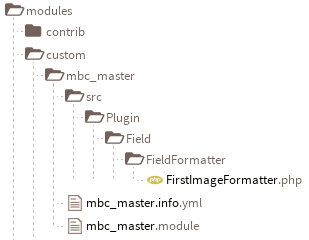
\includegraphics{mbc_master}

% =========================================================================== %
\subsection{Módulo 2 - MBC Review}
Este módulo foi criado com o objetivo de prover um método para o administrador do site enviar e-mail para usuários pedindo Reviews de produtos ou Opiniôes sobre a empresa, prover um link exclusivo para criação destes conteúdos que vai neste e-mail, que reconhece automaticamente o usuário e não publique este conteúdo, deixando-o para moderação do administrador.

% =========================================================================== %
\subsection{Módulo Adaptado - TinyPNG}
Por ser um módulo bem simples que utiliza uma biblioteca externa para fazer a minificação, a adptação deste módulo foi bem simples. Uma função que é executada quando uma entidade (conteúdo) é salva foi utilizada e usada a biblioteca tinify \url{packagist.org/packages/tinify/tinify} para executar a minificação das imagens. Além disso, o módulo adiciona uma página administrativa para ser gerenciada a chave da API do serviço, que pode ser obtida no site \url{https://tinypng.com/}.

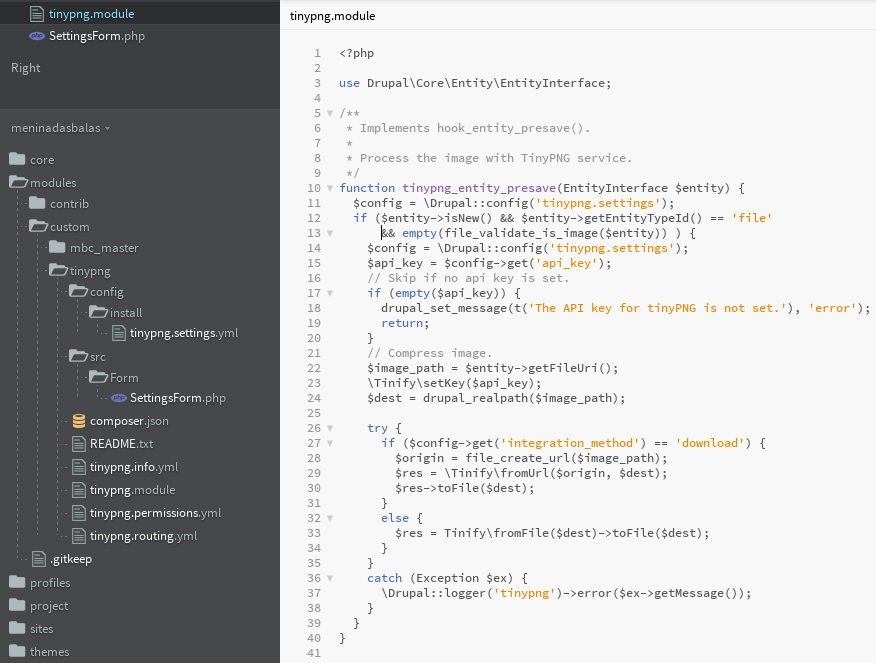
\includegraphics{tinypng2}

% =========================================================================== %
\subsection{Sub-tema - MBC Theme}
Todo front-end do site é construido neste sub-tema. A base é o framework Bootstrap e seu tema para Drupal 8. 

\subsubsection{Gulp}
O automatizador de tarefas Gulp foi utilizado para algumas das principais tarefas de desenvolvimento deste tema como descrito anteriormente e o resultado foi um fluxo de front-end bem mais rápido, sólido e seguro. Todas as ferramentas funcionaram como previsto e todo o código de LESS e Javascript que foram necessários, seguem um padrão de código bem definido e não possuem estruturas inseguras.

\subsubsection{LESS}
Para os arquivos Less, que vão gerar o CSS do site, utilizamos uma estrutura modular, onde cada bloco e página do site tem seu próprio LESS, resultando em arquivos com menos 100 linhas, de facil manutenção e preparados para melhorias no carregamento do CSS pelas páginas do site.

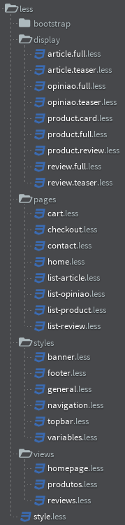
\includegraphics{less}

\subsubsection{Templates Twig}
O Drupal 8 tem um sistema de templates que são utilizados para montar as páginas. Para customizar estes templates, temos que sobrescreve-los. Nosso tema base já possui vários templates sobre-escritos do núcleo e nós nos baseamos nestes para fazer os nossos. Até o momento foram necessários mais de 20 templates e com as melhorias sendo feitas constantemente no site, mais serão criados.

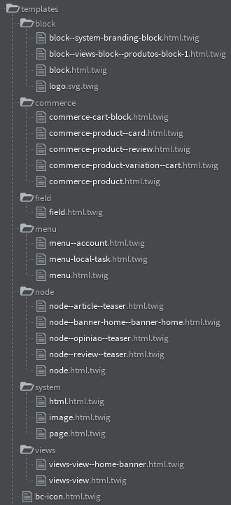
\includegraphics{templates}

% @@@@@@@@@@@@@@@@@@@@@@@@@@@@@@@@@@@@@@@@@@@@@@@@@@@@@@@@@@@@@@@@@@@@@@@@@@@ %
% @@@@@@@@@@@@@@@@@@@@@@@@@@@@@@@@@@@@@@@@@@@@@@@@@@@@@@@@@@@@@@@@@@@@@@@@@@@ %
\section{Performance}

Medimos a performance do site pelo serviço préviamente apresentado chamado GTMetrix. As notas obtidas são bem constantes a cada análise, porém o tempo de resposta do servidor pode mudar significativamente a cada requisição. Configuramos a ferramenta para utilizar um servidor brasileiro, mais especificamente em São Paulo para ser fiel ao publico alvo do site e utilizar o browser Google Chrome, o mais utilizado com 76.87\%\cite{Chrome} dos usuários.

% =========================================================================== %
\subsection{Tempo de Carregamento}
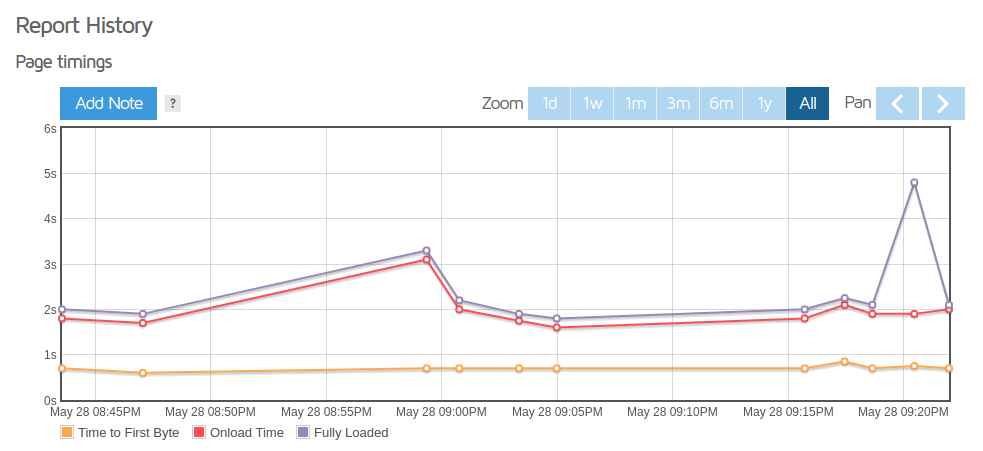
\includegraphics{gtmetrix_history}

Vemos na imagem acima, os tempos de carregamento do site representados pela linha vermelha, tem uma média de 2 segundos. Em apenas um caso este tempo ficou perto dos 3 segundos e em outro, o tempo de carregamento total, que é quando todo o Javascript da página terminou sua execução, foi de aproximados 5 segundo. O tempo entre a requisição da página e o retorno do servidor ficou sempre abaixo do 1 segundo como podemos ver no gráfico pela linha amarela.

% =========================================================================== %
\subsection{Nota, PageSize & Total de Requests}
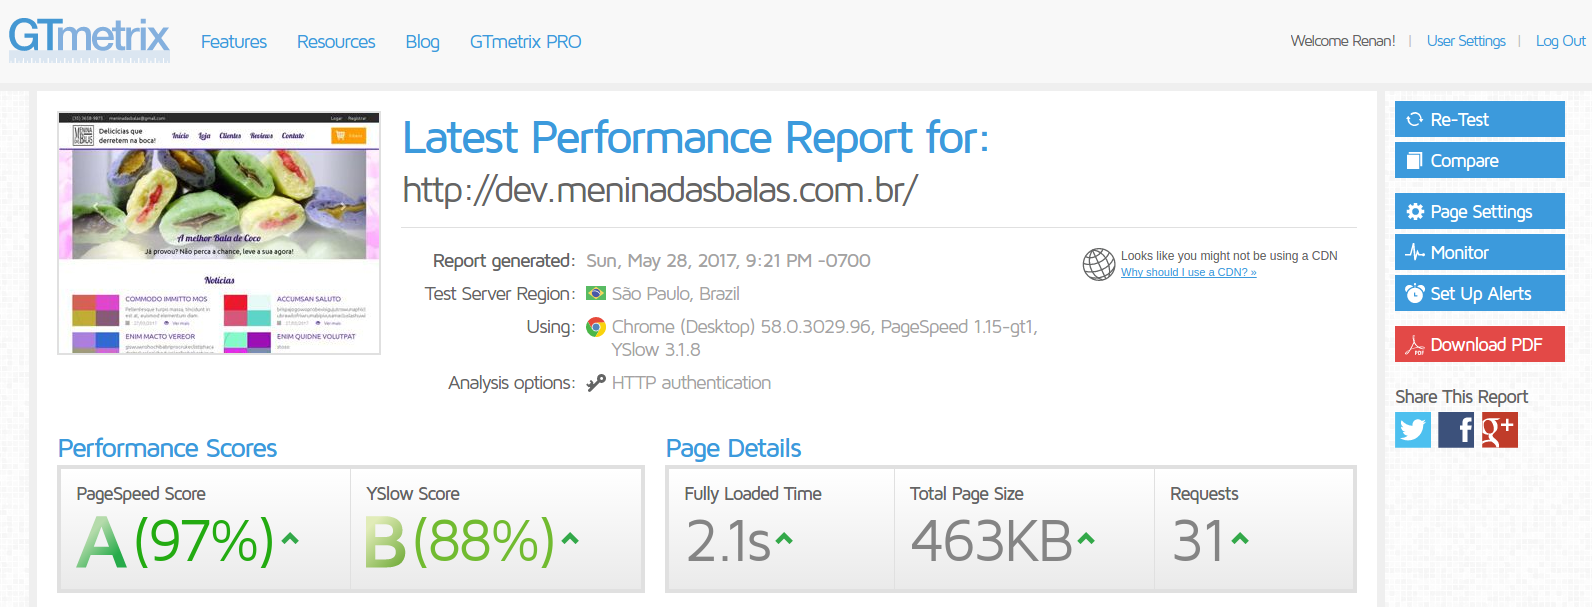
\includegraphics{gtmetrix}

Acima vemos o resultado geral do site na ferramenta GTMetrix. Uma nota excelente foi alcançada no PageSpeed, atingindo 97\% e no YSlow a nota foi boa, chegando a 88\%. Mais adiante veremos o que faltou para estas notas atingirem o 100\%. O tamanho da página também ficou execelente, pois a própria ferramenta diz que a média geral é de 2.52MB e nós conseguimos uma homepage com menos de 0.5MB. Outra informação dada é o número de requests, atingindo 31, com a média geral do GTMetrix sendo 85.

% =========================================================================== %
\subsection{PageSpeed}
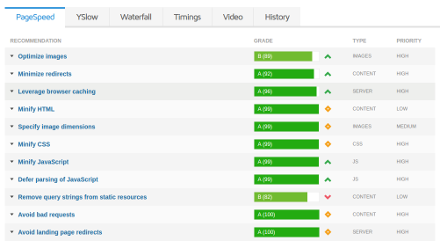
\includegraphics{gtmetrix_pagespeed}
Vamos agora analisar as notas abaixo da nossa média dada pelo PageSpeed e suas dicas para melhorar.

\subsubsection{Optimize Images}
Apesar de já utilizarmos uma ferramenta para minificação das imagens, não foi suficiente para alcançar-mos a melhor nota. A ferramenta acusa que algumas imagens podem ser minificadas ainda mais, entre 3\% e 10\%. Resolvemos não fazer esta melhoria pois a ferramenta atual já funciona bem e a diferença na nota não compensaria o trabalho.

\subsubsection{Minimize Redirects}
Neste quesito, fomos penalizados na nota pois o recurso de Javascript do Google Analytics, adicionado pelo módulo Drupal, é requerido pelo protocolo HTTP e um redirecionamento é feito pelo Google para HTTPS. A diferença dos dois é uma encriptação que aumenta a segurança. Este problema nós só conseguiremos resolver mudando nosso protocolo para HTTPS também, algo que esta na lista de melhorias futuras.

\subsubsection{Leverage browser caching}
Esta é outra penalização por conta do Google Analytics. O mesmo recurso Javascript do item anterior, que é necessário para a ferramenta funcionar, retorna com um header de cache de apenas 2 horas, considerado pouco pelo GTMetrix. Uma solução seria baixar este arquivo e servi-lo do nosso domínio com um cache melhor, porém isso pode prejudicar o uso do Analytics por este ser atualizado constantemente. Assim, escolhemos deixar esta nota como está.

\subsubsection{Remove query strings from static resources}
Os recursos do nosso site, imagens, css e javascript são servidos pelo Drupal e este, utiliza query strings nas urls para controle de cache. Remover estes removeria este controle do sistema sobre os arquivos cacheados, piorando o desempenho em geral. Por este motivo, esta dica também será ignorada.

% =========================================================================== %
\subsection{YSlow}
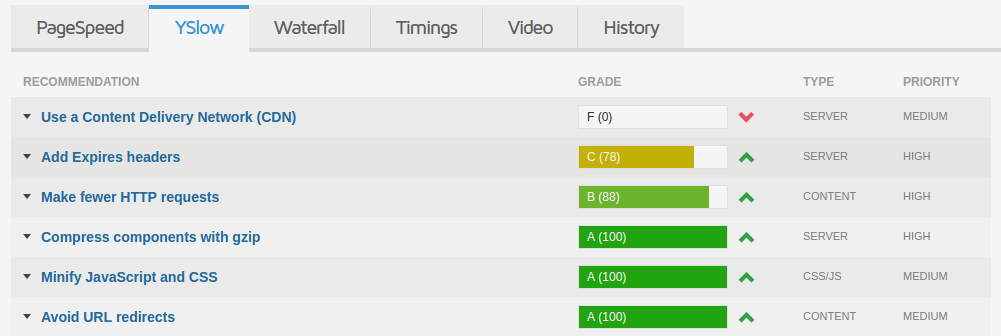
\includegraphics{gtmetrix_yslow}

Agora, analisaremos as dicas da ferramenta YSlow.

\subsubsection{Use a Content Delivery Network}
Neste item, é sugerido que utilizemos um CDN (Rede Central de Distribuição) para servir os arquivos estáticos do site, como CSS, javascript e imagens. Em um CDN, os arquivos ficariam em vários servidores de diferentes localizações e quando uma requisição fosse feita, o servidor mais próximo ou com melhor capacidade seria o escolhido para servir estes arquivos, fazendo com que a velocidade de um site aumente consideravelmente. Por ter um custo alto, este recurso só deve ser implementado em sites muito grandes com milhoês de acessos diários. Pelo nosso site não ter a pretenção de ter um número tão alto de acessos e também por fugir do orçamento do cliente.

\subsubsection{Add expire headers}
Assim como o PageSpeed, o YSlow penaliza por header de cache com tempo de expiração curto. Desta vez dois recursos externos foram citados, o javascript do Google Analytics e o css de fontes do Google Fonts. Novamente, por serem recursos externos, não temos controle sobre o header e deixaremos esta dica sem ação.

\subsubsection{Make fewer HTTP requests}
Esta dica aparece por que o nosso CSS e Javascript foram agregados e separados em 4 arquivos cada. Segundo o YSlow, poderiamos agregar ainda mais e diminuir para um arquivo de cada tipo. Isto não pode ser feito no CSS por que o arquivo não pode ter mais que um número específico de seletores, para manter o suporte ao browser Internet Explorer em versões abaixo do 9. No javascript o problema é o módulo que faz a agregação, que não permite menos de 4 arquivos, que é o considerado ideal pelo criador \cite{AdvAgg}.

% @@@@@@@@@@@@@@@@@@@@@@@@@@@@@@@@@@@@@@@@@@@@@@@@@@@@@@@@@@@@@@@@@@@@@@@@@@@ %
% @@@@@@@@@@@@@@@@@@@@@@@@@@@@@@@@@@@@@@@@@@@@@@@@@@@@@@@@@@@@@@@@@@@@@@@@@@@ %
\section{E-commerce}
O módulo Commerce do Drupal fez todo o trabalho pesado para a construção de um e-commerce. Só resta ao desenvolvedor fazer as configurações, criar campos e customizar o que for preciso. Tudo isto é feito guiado pelas instruções do módulo.

A dificuldade do projeto está focada em duas questões do e-commerce, o método de envio e o método de pagamento. O envio no Brasil é feito pelos Correios, que oferece uma API para consulta de preços. Porem, não temos ainda um módulo que faça esta integração e o desenvolvimento deste daria um trabalho de conclusão por si só. O mesmo acontece com o método de pagamento, as opções nacionais não estão implementadas, nos deixando com os serviços globais, como o que utilizamos, o PayPal.

No front-end, vários templates e muito CSS ajudam a melhorar o estilo das páginas, que não possuêm um tema 'out-of-the-box'. Tudo isso fez com que o resultado final seja um e-commerce simples, porém robusto e que se trabalhado mais algum tempo, tem um grande potêncial.

% @@@@@@@@@@@@@@@@@@@@@@@@@@@@@@@@@@@@@@@@@@@@@@@@@@@@@@@@@@@@@@@@@@@@@@@@@@@ %
% @@@@@@@@@@@@@@@@@@@@@@@@@@@@@@@@@@@@@@@@@@@@@@@@@@@@@@@@@@@@@@@@@@@@@@@@@@@ %
\section{Final}

O resultado final pode ser verificado nas imagens no apêndice \ref{appendix:site} ou pela URL:

\begin{center}
  http://meninadasbalas.com.br/
\end{center}

Todo o código feito pode ser visto e baixado no repositório publico do projeto no Github na URL:

\begin{center}
  https://github.com/renanmfd/meninadasbalas
\end{center}

\chapter{Discussão}

\sectuin{O que faltou?}


\section{Melhorias}

\subsection{Minificação}
Mudar o serviço utilizado para minificação das imagens do site, ajudaria a melhorar a nota do site e sua performance, o que traria um benefício na indexação por motores de busca. As alternativas são OptiPNG e JpegOptim, ambas ferramentas de código livre. A dificuldade estaria em integra-las com o Drupal, pois ambas são utilizadas em linha de comando.

\subsection{Funções Acicionais no E-commerce}
Para facilitar o rasteamento do pedido pelo usuário, fariamos uma área do cliente com todos os serviços relativos ao pedido como por exemplo rastreamento da encomenda, status do pagamento e histórico de pedidos.

\subsection{Calculadora de Frete}
Outro serviço interessante para se implementar, seria uma página de calculo de frete, onde o usuário entra com informações como quantidade de balas e cep em um formulario e tem como resposta as opções de frete e seus preços.

\subsection{Design}
A mudança mais necessária que vemos é um novo design. Por maior que seja o esforço feito, o design, que é um das principais características de um website, não ficou muito bom. Um trabalho de re-design seria extramamente importante e se possível feito por um profissional, que saiba valorizar os principais pontos do site e o faça de maneira fluida e harmoniosa.

\chapter{Conclusão}

Pela falta de interesse momentâneo do cliente, o site não foi divulgado e sua função e-commerce está desabilitada. Por este motivo não pudemos resultados relevantes coletados de SEO, que necessita um site minimamente divulgado. Apesar disto, mesmo sem um conteúdo relevante, aparecer na primeira página em uma busca mostra que estamos no caminho certo e que quando colocar-mos o site 100\% online com um conteúdo bem produzido e com algumas campanhas de marketing, ele será muito melhor indexado.

A performance obtida foi altamente satisfatória, acima do esperado e atingindo o objetivo definido. A surpresa fica pelo tempo de resposta do servidor, que apesar de ser compartilhado e de baixo custo, mostrou-se bem rápido e capaz. A ferramenta GTMetrix ajudou na medição e também com dicas nos vários teste que foram realizados durante o desenvolvimento, sendo de suma importância para o projeto.

O e-commerce, apesar de não abilitado, funcionou muito bem nos testes e é esperado que quando colocado a disposição do publico, funcione sem problemas. Até o momento não foi testada uma compra real, com um número de cartão válido, somente compras com cartões de testes providos pelo PayPal, que em teoria seriam suficientes. As funções de envio de e-mail ao final da compra foram testadas e funcionam sem problemas. No geral, o e-commerce funciona como esperado, mas ainda sim, tem muito a melhorar.

Como dito no capitulo anterior, um ponto que não teve um resultado satisfatório foi o design. Apesar disto, vejo que a dificuldade de ter este ponto re-feito é mínima e o mais importante é que está funcional e bem programado.

Finalmente, o projeto como um todo, teve um resultado satisfatório na maioria do pontos dados como objetivos, superando as espectatívas em alguns. Foi um objeto bastante complexo, por ter passar por várias áreas de um sistema web, como servidor, back-end, front-end e SEO, e por isso, bastante valioso para o aprendizado.

%\chapter{Resultado}

\section{Resultado I}

TODO

\section{Resultado II}

TODO

TODO Schema.org

%\chapter{Discussão}

\section{Melhorias}

\subsection{Minificação}
Mudar o serviço utilizado para minificação das imagens do site, ajudaria a melhorar a nota do site e sua performance, o que traria um benefício na indexação por motores de busca. As alternativas são OptiPNG e JpegOptim, ambas ferramentas de código livre. A dificuldade estaria em integrá-las com o Drupal, pois ambas são utilizadas em linha de comando.

\subsection{Funções Acicionais no E-commerce}
Para facilitar o rasteamento do pedido pelo usuário, fariamos uma área do cliente com todos os serviços relativos ao pedido como, por exemplo, rastreamento da encomenda, status do pagamento e histórico de pedidos.

\subsection{Calculadora de Frete}
Outro serviço interessante para se implementar, seria uma página de cálculo de frete, onde o usuário entra com informações como quantidade de balas e CEP em um formulário e tem como resposta as opções de frete e seus preços.

\subsection{Design}
A mudança mais necessária que vemos é um novo design. Por maior que seja o esforço feito, o design, que é um das principais características de um website, não ficou muito bom. Um trabalho de \textit{re-design} seria extramamente bem vindo e se possível feito por um profissional, que saiba como valorizar os principais pontos do site e o faça de maneira fluida e harmoniosa.

%\chapter{Conclusão}

Pela falta de interesse momentâneo do cliente, o site não foi divulgado e sua função e-commerce está desabilitada. Por este motivo não pudemos resultados relevantes coletados de SEO, que necessita um site minimamente divulgado. Apesar disto, mesmo sem um conteúdo relevante, aparecer na primeira página em uma busca mostra que estamos no caminho certo e que quando colocar-mos o site 100\% online com um conteúdo bem produzido e com algumas campanhas de marketing, ele será muito melhor indexado.

A performance obtida foi altamente satisfatória, acima do esperado e atingindo o objetivo definido. A surpresa fica pelo tempo de resposta do servidor, que apesar de ser compartilhado e de baixo custo, mostrou-se bem rápido e capaz. A ferramenta GTMetrix ajudou na medição e também com dicas nos vários teste que foram realizados durante o desenvolvimento, sendo de suma importância para o projeto.

O e-commerce, apesar de não abilitado, funcionou muito bem nos testes e é esperado que quando colocado a disposição do publico, funcione sem problemas. Até o momento não foi testada uma compra real, com um número de cartão válido, somente compras com cartões de testes providos pelo PayPal, que em teoria seriam suficientes. As funções de envio de e-mail ao final da compra foram testadas e funcionam sem problemas. No geral, o e-commerce funciona como esperado, mas ainda sim, tem muito a melhorar.

Como dito no capitulo anterior, um ponto que não teve um resultado satisfatório foi o design. Apesar disto, vejo que a dificuldade de ter este ponto re-feito é mínima e o mais importante é que está funcional e bem programado.

Finalmente, o projeto como um todo, teve um resultado satisfatório na maioria do pontos dados como objetivos, superando as espectatívas em alguns. Foi um objeto bastante complexo, por ter passar por várias áreas de um sistema web, como servidor, back-end, front-end e SEO, e por isso, bastante valioso para o aprendizado.

% ----------------------------------------------------------
% ELEMENTOS PÓS-TEXTUAIS
% ----------------------------------------------------------
\postextual
% ----------------------------------------------------------

% ----------------------------------------------------------
% Referências bibliográficas
% ----------------------------------------------------------
\bibliography{monografia}

% ----------------------------------------------------------
% Glossário
% ----------------------------------------------------------
%
% Consulte o manual da classe abntex2 para orientações sobre o glossário.
%
%\glossary

% ----------------------------------------------------------
% Apêndices
% ----------------------------------------------------------

% ---
% Inicia os apêndices
% ---
\begin{apendicesenv}

% Imprime uma página indicando o início dos apêndices
\partapendices
% ----------------------------------------------------------
\chapter{Quisque libero justo}
% ----------------------------------------------------------

\end{apendicesenv}
% ---

\end{document}
